\documentclass[10pt,a4paper]{report}
\usepackage[utf8]{inputenc}
\usepackage[russian]{babel}
\usepackage{amsmath}
\usepackage{amsfonts}
\usepackage{amssymb}
\usepackage{graphicx}
\renewcommand{\thesection}{\arabic{section}}
\setcounter{totalnumber}{10}
\setcounter{topnumber}{10}
\setcounter{bottomnumber}{10}
\renewcommand{\topfraction}{1}
\renewcommand{\textfraction}{0}
\author{Никитина Анна}
\title{Лабораторная работа №4.\\
	Утилита для исследования сети и сканер портов Nmap}
\begin{document}
\maketitle
\tableofcontents
\pagebreak

\section{Цель работы}
Изучить возможности утилиты Nmap на различных примерах.
\section{Ход работы}
Для выполнения лабораторной работы понадобятся две виртуальные машины. Metasploitable2 -виртуальная машина, содержащая различные уязвимости. Kali Linux - виртуальная машина, способная сканировать и находить уязвимости. Вышеуказанные машины необходимо объединить в общую сеть.
Определим IP-адрес на машине Kali Linux 
\begin{verbatim}
root@kali:~# ifconfig -a
eth0: flags=4163<UP,BROADCAST,RUNNING,MULTICAST>  mtu 1500
        inet 192.168.0.102  netmask 255.255.255.0  broadcast 192.168.0.255
        inet6 fe80::a00:27ff:fe9b:2f3f  prefixlen 64  scopeid 0x20<link>
\end{verbatim}
И на машине Metasploitable2 
\begin{verbatim}
root@kali:~# ifconfig -a
eth0: flags=4163<UP,BROADCAST,RUNNING,MULTICAST>  mtu 1500
        inet 192.168.0.103  netmask 255.255.255.0  broadcast 192.168.0.255
        inet6 fe80::a00:27ff:fe9b:2f3f  prefixlen 64  scopeid 0x20<link>
\end{verbatim}
\subsection{Поиск активных хостов}
Для поиска активных хостов указываем флаг -sP и  адрес подсети  192.168.0.*
\begin{verbatim}
root@kali:~# nmap -sP 192.168.0.*

Starting Nmap 7.01 ( https://nmap.org ) at 2016-03-27 14:48 EDT
Nmap scan report for 192.168.0.1
Host is up (0.0057s latency).
MAC Address: 1C:7E:E5:3E:AF:10 (D-Link International)
Nmap scan report for 192.168.0.100
Host is up (0.00027s latency).
MAC Address: E0:B9:A5:1C:8A:33 (AzureWave Technology)
Nmap scan report for 192.168.0.103
Host is up (0.00081s latency).
MAC Address: 08:00:27:94:82:93 (Oracle VirtualBox virtual NIC)
Nmap scan report for 192.168.0.102
Host is up.
Nmap done: 256 IP addresses (4 hosts up) scanned in 28.20 seconds
\end{verbatim}
\subsection{Определение открытых портов}
Для определения открытых портов утилите достаточно передать адрес хоста.
\begin{verbatim}
root@kali:~# nmap  192.168.0.103

Starting Nmap 7.01 ( https://nmap.org ) at 2016-03-27 15:23 EDT
Nmap scan report for 192.168.0.103
Host is up (0.00045s latency).
Not shown: 977 closed ports
PORT     STATE SERVICE
21/tcp   open  ftp
22/tcp   open  ssh
23/tcp   open  telnet
25/tcp   open  smtp
53/tcp   open  domain
80/tcp   open  http
111/tcp  open  rpcbind
139/tcp  open  netbios-ssn
445/tcp  open  microsoft-ds
512/tcp  open  exec
513/tcp  open  login
514/tcp  open  shell
1099/tcp open  rmiregistry
1524/tcp open  ingreslock
2049/tcp open  nfs
2121/tcp open  ccproxy-ftp
3306/tcp open  mysql
5432/tcp open  postgresql
5900/tcp open  vnc
6000/tcp open  X11
6667/tcp open  irc
8009/tcp open  ajp13
8180/tcp open  unknown
MAC Address: 08:00:27:94:82:93 (Oracle VirtualBox virtual NIC)

Nmap done: 1 IP address (1 host up) scanned in 13.33 seconds
\end{verbatim}
Также существуют флаги -sT для определения открытх TCP-портов, -sU для определения UDP-портов.
\subsection{Определение версии сервисов}
Для определения версий сервисов необходимо указать флаг -sV.
\begin{verbatim}
root@kali:~# nmap -sV 192.168.0.103

Starting Nmap 7.01 ( https://nmap.org ) at 2016-03-27 15:32 EDT
Nmap scan report for 192.168.0.103
Host is up (0.00024s latency).
Not shown: 977 closed ports
PORT     STATE SERVICE     VERSION
21/tcp   open  ftp         vsftpd 2.3.4
22/tcp   open  ssh         OpenSSH 4.7p1 Debian 8ubuntu1 (protocol 2.0)
23/tcp   open  telnet      Linux telnetd
25/tcp   open  smtp        Postfix smtpd
53/tcp   open  domain      ISC BIND 9.4.2
80/tcp   open  http        Apache httpd 2.2.8 ((Ubuntu) DAV/2)
111/tcp  open  rpcbind     2 (RPC #100000)
139/tcp  open  netbios-ssn Samba smbd 3.X (workgroup: WORKGROUP)
445/tcp  open  netbios-ssn Samba smbd 3.X (workgroup: WORKGROUP)
512/tcp  open  exec        netkit-rsh rexecd
513/tcp  open  login?
514/tcp  open  tcpwrapped
1099/tcp open  rmiregistry GNU Classpath grmiregistry
1524/tcp open  shell       Metasploitable root shell
2049/tcp open  nfs         2-4 (RPC #100003)
2121/tcp open  ftp         ProFTPD 1.3.1
3306/tcp open  mysql       MySQL 5.0.51a-3ubuntu5
5432/tcp open  postgresql  PostgreSQL DB 8.3.0 - 8.3.7
5900/tcp open  vnc         VNC (protocol 3.3)
6000/tcp open  X11         (access denied)
6667/tcp open  irc         Unreal ircd
8009/tcp open  ajp13       Apache Jserv (Protocol v1.3)
8180/tcp open  http        Apache Tomcat/Coyote JSP engine 1.1
MAC Address: 08:00:27:94:82:93 (Oracle VirtualBox virtual NIC)
Service Info: Hosts:  metasploitable.localdomain, localhost, irc.Metasploitable.LAN; OSs: Unix, Linux; CPE: cpe:/o:linux:linux_kernel

Service detection performed. Please report any incorrect results at https://nmap.org/submit/ .
Nmap done: 1 IP address (1 host up) scanned in 31.98 seconds
\end{verbatim}
\subsection{Изучение файлов nmap-services, nmap-os-db, nmap-service-probes}
Файл \textbf{nmap-services} представляет собой список, каждая строка которого состоит из имени порта, соответствующего ему номера и протокола. Дпалее число, представляющее собой вероятность того, что порт является открытым. Большинство строк имеют также комментарии.

\begin{verbatim}
mit-ml-dev	83/tcp	0.000539	# MIT ML Device
mit-ml-dev	83/udp	0.001203	# MIT ML Device
ctf	84/tcp	0.000276	# Common Trace Facility
ctf	84/udp	0.000610	# Common Trace Facility
mit-ml-dev	85/tcp	0.000690	# MIT ML Device
mit-ml-dev	85/udp	0.000610	# MIT ML Device
mfcobol	86/tcp	0.000138	# Micro Focus Cobol
mfcobol	86/udp	0.000824	# Micro Focus Cobol
\end{verbatim}
Файл \textbf{nmap-os-db} содержит примеры ответов различных операционных систем при сканировании Nmap. Он разделен на блоки, называемые Fingerprint, каждый из которых содержат  название операционной системы, ее общую классификацию, и данные от нее. 
\begin{verbatim}
# 3Com OfficeConnect 3CR858-91 Software version V1.13-168 (Mar 21 2008 11:57:49)
Fingerprint 3Com OfficeConnect 3CR858-91 router
Class 3Com | embedded || router
CPE cpe:/h:3com:officeconnect_3cr858-91 auto
SEQ(SP=0-5%GCD=B|16|21|2C|37%ISR=30-3A%TI=I%CI=I%II=I%SS=S%TS=U)
OPS(O1=M578%O2=M578%O3=M280%O4=M578%O5=M218%O6=M109)
WIN(W1=1770%W2=1770%W3=1770%W4=1770%W5=1770%W6=1770)
ECN(R=Y%DF=Y%T=3B-45%TG=40%W=1770%O=M578%CC=N%Q=)
T1(R=Y%DF=Y%T=3B-45%TG=40%S=O%A=O|S+%F=AS%RD=0%Q=)
T2(R=N)
T3(R=N)
\end{verbatim}
Файл \textbf{nmap-service-probes} представляет из себя список, содержащий сигнатуры для определения различных сервисов. Используются несколько директив, некоторые из них:
\begin{itemize}
\item Probe <protocol> <probename> <probestring> \\ Директива Probe содержит строку, необходимую для отправки при распознавании сервиса.
\item match <service> <pattern> [<versioninfo>]\\
Директива match необходима при распознавании сервиса на основе ответов на строку, отправленную предыдущей директивой Probe.
\item ports <portlist>\\
Директива ports содержит порты сервиса.
\item rarity <value between 1 and 9> \\
Директива rarity указывает частоту, с которой от сервиса можно ожидать возвращения корректных результатов.
\end{itemize}
Пример из файла nmap-service-probes
\begin{verbatim}
Probe TCP Radmin q|\x01\x00\x00\x00\x01\x00\x00\x00\x08\x08|
ports 4899,9001
rarity 8
match fcgiwrap m|^\x01\x0b\0\0\0\x08\0\0\0\0\0\0\0\0\0\0$| p/fcgiwrap/
match radmin m|^\x01\x00\x00\x00\x25\x09\x00\x01\x10\x08\x01\x00\x09\x08| p/Famatech Radmin/ v/2.X/ i/Windows Authentication/ o/Windows/ cpe:/a:famatech:radmin:2/ cpe:/o:microsoft:windows/a
match radmin m|^\x01\x00\x00\x00\x25\x0a\x00\x01\x10\x08\x01\x00\x0a\x08| p/Famatech Radmin/ v/2.X/ i/Radmin Authentication/ o/Windows/ cpe:/a:famatech:radmin:2/ cpe:/o:microsoft:windows/a
match radmin m|^\x01\x00\x00\x00\x25\x00\x00\x02\x12\x08\x02\x00\x00\x0a| p/Famatech Radmin/ v/3.X/ i/Radmin Authentication/ o/Windows/ cpe:/a:famatech:radmin:3/ cpe:/o:microsoft:windows/a
match radmin m|^\x01\x00\x00\x00\x25\x71\x00\x02\x12\x08\x02\x00\x71\x0a| p/Famatech Radmin/ v/3.X/ i/Windows Authentication/ o/Windows/ cpe:/a:famatech:radmin:3/ cpe:/o:microsoft:windows/a
\end{verbatim}
\subsection{Добавление собственной сигнатуры в файл nmap-service-probes}
Создадим простейший сервер, который будет работать на 8089 порту.
\begin{verbatim}
#include <sys/socket.h> 
#include <netinet/in.h> 
#include <arpa/inet.h> 
#include <stdio.h> 
#include <stdlib.h> 
#include <string.h> 
#include <unistd.h> 
#define DEF_PORT 8089 

int main(int argc, char** argv) 
{ 
char str[100];
char *sendStr="\x48\x65\x6c\x6c\x6f";
struct sockaddr_in listenerInfo; 
listenerInfo.sin_family = AF_INET; 
listenerInfo.sin_port = htons(DEF_PORT); 
listenerInfo.sin_addr.s_addr = htonl(INADDR_ANY); 
int listener = socket(AF_INET,SOCK_STREAM,0); 
if(listener < 0) { 
perror("Can't create socket to listen: "); 
exit(1); 
} 
int res = bind(listener,(struct sockaddr *) &listenerInfo,sizeof(listenerInfo)); 
if(res < 0) { 
perror("Can't bind socket"); 
exit(1); 
} 
res = listen(listener,5); 
if(res) { 
perror("Erro while listening:"); 
exit(1); 
}
int client = accept(listener,NULL,NULL);
while(1)
{
bzero( str, 100);
recv(client,str, 100, 0); 
printf("Message from client - %s",str);
send(client, sendStr, (int)strlen(sendStr), 0);
}
return 0; 
}
\end{verbatim}
Добавим в nmap-service-probes строки о созданном сервисе.  \\
Для распознавания сервиса отправлется строка 'HelloServer!', в ответ ожидается строка 'Hello'. Порт сервиса 8089.
\begin{verbatim}
Probe TCP MyServer q|HelloServer!|
rarity 1
ports 8089
match MyServer m|\x48\x65\x6c\x6c\x6f| v/0.1/
\end{verbatim}

Запустим сервис на машине Metasploitable2 И проверим с помощью nmap наличие сервиса, указав IP-адрес машины 192.168.0.103. 


\begin{verbatim}
root@kali:~# nmap 192.168.0.103 -sV 
Starting Nmap 7.01 ( https://nmap.org ) at 2016-04-02 05:57 EDT
Nmap scan report for 192.168.0.103
Host is up (0.00058s latency).
Not shown: 977 closed ports
PORT     STATE SERVICE     VERSION
21/tcp   open  ftp         vsftpd 2.3.4
.....
5900/tcp open  vnc         VNC (protocol 3.3)
6000/tcp open  X11         (access denied)
6667/tcp open  irc         Unreal ircd
8009/tcp open  ajp13       Apache Jserv (Protocol v1.3)
8180/tcp open  http        Apache Tomcat/Coyote JSP engine 1.1
8089/tcp open  MyServer    0.1
MAC Address: 08:00:27:94:82:93 (Oracle VirtualBox virtual NIC)
Service Info: Hosts:  metasploitable.localdomain, localhost, irc.Metasploitable.LAN; OSs: Unix, Linux; CPE: cpe:/o:linux:linux_kernel

Service detection performed. Please report any incorrect results at https://nmap.org/submit/ .
Nmap done: 1 IP address (1 host up) scanned in 29.93 seconds
\end{verbatim}
Созданный сервис успешно распознан, названия и версия при этом указываются.
\subsection{Сохранение вывода утилиты в формате XML}
Для сохранения вывода утилиты в файле xml необходимо указать флаг -oX, после которого имя файла (в примере ниже example.xml).
\begin{verbatim}
root@kali:~# nmap 192.168.0.103 -oX example.xml
\end{verbatim}
Просмотрим файл example.xml. В него была записана информация о сервисах хоста 192.168.0.103 в формате xml.
\begin{verbatim}
<?xml version="1.0" encoding="UTF-8"?>
<!DOCTYPE nmaprun>
<?xml-stylesheet href="file:///usr/bin/../share/nmap/nmap.xsl" type="text/xsl"?>
<!-- Nmap 7.01 scan initiated Sat Apr  2 07:42:49 2016 as: nmap -oX xml.txt 192.168.0.103 -->
<nmaprun scanner="nmap" args="nmap -oX xml.txt 192.168.0.103" start="1459597369" startstr="Sat Apr  2 07:42:49 2016" version="7.01" xmloutputversion="1.04">
<scaninfo type="syn" protocol="tcp" numservices="1000" services="1,3-4,6-7,9,13,17,19-26,30,32-33,37,42-43,49,53,70,79-85,88-90,99-100,106,109-111,113,119,125,135,139,143-144,146,161,163,179,199,211-212,222,254-256,259,264,280,301,306,311,340,366,389,406-407,416-417,425,427,443-445,458,464-465,481,497,500,512-515,524,541,543-545,548,554-555,563,587,593,616-617,625,631,636,646,648,666-668,683,687,691,700,705,711,714,720,722,726,749,765,777,783,787,800-801,808,843,873,880,888,898,900-903,911-912,981,987,990,992-993,995,999-1002,1007,1009-1011,1021-1100,1102,1104-1108,1110-1114,1117,1119,1121-1124,1126,1130-1132,1137-1138,1141,1145,1147-1149,1151-1152,1154,1163-1166,1169,1174-1175,1183,1185-1187,1192,1198-1199,1201,1213,1216-1218,1233-1234,1236,1244,1247-1248,1259,1271-1272,1277,1287,1296,1300-1301,1309-1311,1322,1328,1334,1352,1417,1433-1434,1443,1455,1461,1494,1500-1501,1503,1521,1524,1533,1556,1580,1583,1594,1600,1641,1658,1666,1687-1688,1700,1717-1721,1723,1755,1761,1782-1783,1801,1805,1812,1839-1840,1862-1864,1875,1900,1914,1935,1947,1971-1972,1974,1984,1998-2010,2013,2020-2022,2030,2033-2035,2038,2040-2043,2045-2049,2065,2068,2099-2100,2103,2105-2107,2111,2119,2121,2126,2135,2144,2160-2161,2170,2179,2190-2191,2196,2200,2222,2251,2260,2288,2301,2323,2366,2381-2383,2393-2394,2399,2401,2492,2500,2522,2525,2557,2601-2602,2604-2605,2607-2608,2638,2701-2702,2710,2717-2718,2725,2800,2809,2811,2869,2875,2909-2910,2920,2967-2968,2998,3000-3001,3003,3005-3007,3011,3013,3017,3030-3031,3052,3071,3077,3128,3168,3211,3221,3260-3261,3268-3269,3283,3300-3301,3306,3322-3325,3333,3351,3367,3369-3372,3389-3390,3404,3476,3493,3517,3527,3546,3551,3580,3659,3689-3690,3703,3737,3766,3784,3800-3801,3809,3814,3826-3828,3851,3869,3871,3878,3880,3889,3905,3914,3918,3920,3945,3971,3986,3995,3998,4000-4006,4045,4111,4125-4126,4129,4224,4242,4279,4321,4343,4443-4446,4449,4550,4567,4662,4848,4899-4900,4998,5000-5004,5009,5030,5033,5050-5051,5054,5060-5061,5080,5087,5100-5102,5120,5190,5200,5214,5221-5222,5225-5226,5269,5280,5298,5357,5405,5414,5431-5432,5440,5500,5510,5544,5550,5555,5560,5566,5631,5633,5666,5678-5679,5718,5730,5800-5802,5810-5811,5815,5822,5825,5850,5859,5862,5877,5900-5904,5906-5907,5910-5911,5915,5922,5925,5950,5952,5959-5963,5987-5989,5998-6007,6009,6025,6059,6100-6101,6106,6112,6123,6129,6156,6346,6389,6502,6510,6543,6547,6565-6567,6580,6646,6666-6669,6689,6692,6699,6779,6788-6789,6792,6839,6881,6901,6969,7000-7002,7004,7007,7019,7025,7070,7100,7103,7106,7200-7201,7402,7435,7443,7496,7512,7625,7627,7676,7741,7777-7778,7800,7911,7920-7921,7937-7938,7999-8002,8007-8011,8021-8022,8031,8042,8045,8080-8090,8093,8099-8100,8180-8181,8192-8194,8200,8222,8254,8290-8292,8300,8333,8383,8400,8402,8443,8500,8600,8649,8651-8652,8654,8701,8800,8873,8888,8899,8994,9000-9003,9009-9011,9040,9050,9071,9080-9081,9090-9091,9099-9103,9110-9111,9200,9207,9220,9290,9415,9418,9485,9500,9502-9503,9535,9575,9593-9595,9618,9666,9876-9878,9898,9900,9917,9929,9943-9944,9968,9998-10004,10009-10010,10012,10024-10025,10082,10180,10215,10243,10566,10616-10617,10621,10626,10628-10629,10778,11110-11111,11967,12000,12174,12265,12345,13456,13722,13782-13783,14000,14238,14441-14442,15000,15002-15004,15660,15742,16000-16001,16012,16016,16018,16080,16113,16992-16993,17877,17988,18040,18101,18988,19101,19283,19315,19350,19780,19801,19842,20000,20005,20031,20221-20222,20828,21571,22939,23502,24444,24800,25734-25735,26214,27000,27352-27353,27355-27356,27715,28201,30000,30718,30951,31038,31337,32768-32785,33354,33899,34571-34573,35500,38292,40193,40911,41511,42510,44176,44442-44443,44501,45100,48080,49152-49161,49163,49165,49167,49175-49176,49400,49999-50003,50006,50300,50389,50500,50636,50800,51103,51493,52673,52822,52848,52869,54045,54328,55055-55056,55555,55600,56737-56738,57294,57797,58080,60020,60443,61532,61900,62078,63331,64623,64680,65000,65129,65389"/>
<verbose level="0"/>
<debugging level="0"/>
<host starttime="1459597369" endtime="1459597382"><status state="up" reason="arp-response" reason_ttl="0"/>
<address addr="192.168.0.103" addrtype="ipv4"/>
<address addr="08:00:27:94:82:93" addrtype="mac" vendor="Oracle VirtualBox virtual NIC"/>
<hostnames>
</hostnames>
<ports><extraports state="closed" count="977">
<extrareasons reason="resets" count="977"/>
</extraports>
<port protocol="tcp" portid="21"><state state="open" reason="syn-ack" 
reason_ttl="64"/><service name="ftp" method="table" conf="3"/></port>
<port protocol="tcp" portid="22"><state state="open"
 reason="syn-ack" reason_ttl="64"/><service name="ssh" method="table" conf="3"/></port>
<port protocol="tcp" portid="23"><state state="open"
 reason="syn-ack" reason_ttl="64"/><service name="telnet" method="table" conf="3"/></port>
<port protocol="tcp" portid="25"><state state="open"
 reason="syn-ack" reason_ttl="64"/><service name="smtp" method="table" conf="3"/></port>
<port protocol="tcp" portid="53"><state state="open"
 reason="syn-ack" reason_ttl="64"/><service name="domain" method="table" conf="3"/></port>
<port protocol="tcp" portid="80"><state state="open"
 reason="syn-ack" reason_ttl="64"/><service name="http" method="table" conf="3"/></port>
...
<port protocol="tcp" portid="514"><state state="open"
 reason="syn-ack" reason_ttl="64"/><service name="shell" method="table" conf="3"/></port>
<port protocol="tcp" portid="1099"><state state="open"
 reason="syn-ack" reason_ttl="64"/><service name="rmiregistry" method="table" conf="3"/></port>
<port protocol="tcp" portid="1524"><state state="open"
 reason="syn-ack" reason_ttl="64"/><service name="ingreslock" method="table" conf="3"/></port>
<port protocol="tcp" portid="2049"><state state="open"
 reason="syn-ack" reason_ttl="64"/><service name="nfs" method="table" conf="3"/></port>
<port protocol="tcp" portid="2121"><state state="open"
 reason="syn-ack" reason_ttl="64"/><service name="ccproxy-ftp" method="table" conf="3"/></port>
<port protocol="tcp" portid="3306"><state state="open"
 reason="syn-ack" reason_ttl="64"/><service name="mysql" method="table" conf="3"/></port>
<port protocol="tcp" portid="5432"><state state="open"
 reason="syn-ack" reason_ttl="64"/><service name="postgresql" method="table" conf="3"/></port>
<port protocol="tcp" portid="5900"><state state="open"
 reason="syn-ack" reason_ttl="64"/><service name="vnc" method="table" conf="3"/></port>
<port protocol="tcp" portid="6000"><state state="open"
 reason="syn-ack" reason_ttl="64"/><service name="X11" method="table" conf="3"/></port>
<port protocol="tcp" portid="6667"><state state="open"
 reason="syn-ack" reason_ttl="64"/><service name="irc" method="table" conf="3"/></port>
<port protocol="tcp" portid="8009"><state state="open"
 reason="syn-ack" reason_ttl="64"/><service name="ajp13" method="table" conf="3"/></port>
<port protocol="tcp" portid="8180"><state state="open"
 reason="syn-ack" reason_ttl="64"/><service name="unknown" method="table" conf="3"/></port>
</ports>
<times srtt="448" rttvar="260" to="100000"/>
</host>
<runstats><finished time="1459597382" timestr="Sat Apr  2 07:43:02 2016" elapsed="13.42" summary="Nmap done at Sat Apr  2 07:43:02 2016; 1 IP address (1 host up) scanned in 13.42 seconds" exit="success"/><hosts up="1" down="0" total="1"/>
</runstats>
</nmaprun>
\end{verbatim}
\subsection{Исследование с использованием утилиты WireShark}
Запустим утилиту WireShark, после чего просканируем хост 192.168.0.103.
\begin{verbatim}
root@kali:~# nmap 192.168.0.103
\end{verbatim}
Как показано на рисунке \ref{ris:image1}. Изначально nmap посылат на существующие порты TCP-пакеты с установленным флагом SYN, что означает установление соединения. Если при этом сканируемый порт отправляет ответ с установленными флагами [RST, ACK], значит соединение невозможно - порт закрыт.  \\
\begin{figure}[ht]	\center{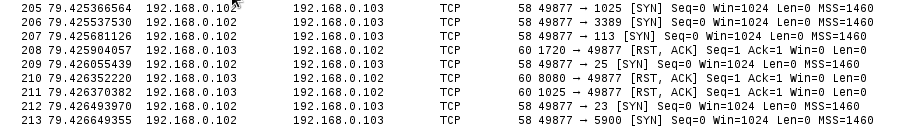
\includegraphics[width=1.4\linewidth]{img/1}}
\caption{Вывод утилиты WireShark.}\label{ris:image1}
\end{figure} \\
Если после отправки TCP-пакета с флагом SYN сканируемый порт отправляет ответ также с установленным флагом SYN, это означает, что заданый порт открыт. Пример показан на рисунке \ref{ris:image2} .  
\begin{figure}[ht]	\center{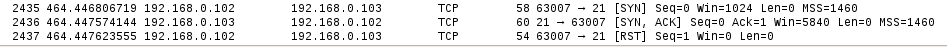
\includegraphics[width=1.4\linewidth]{img/2}}
\caption{Вывод утилиты WireShark.}\label{ris:image2}
\end{figure}
\subsection{Использвоание db\_nmap из состава metasploit-framewor}
Первым шагом надо запустить postgresql сервер.  После чего создать и инициализировать базу данных командой msfdb init. И запустить консоль  msfconsole.
\begin{verbatim}
root@kali:~# service postgresql start
root@kali:~# msfdb init
Creating database user 'msf'
Enter password for new role: 
Enter it again: 
Creating databases 'msf' and 'msf_test'
Creating configuration file in /usr/share/metasploit-framework/config/database.yml
Creating initial database schema
root@kali:~# msfconsole
\end{verbatim}
После чего доступна команда db\_nmap, которая имеет ту же функциональность, что и команда nmap. Однако в этом случае результаты сканирования будут автоматически сохранены в базе данных. 
\begin{verbatim}
msf > db_nmap 192.168.0.103 -p 21
[*] Nmap: Starting Nmap 7.01 ( https://nmap.org ) at 2016-04-02 09:06 EDT
[*] Nmap: Nmap scan report for 192.168.0.103
[*] Nmap: Host is up (0.00095s latency).
[*] Nmap: PORT   STATE SERVICE
[*] Nmap: 21/tcp open  ftp
[*] Nmap: MAC Address: 08:00:27:94:82:93 (Oracle VirtualBox virtual NIC)
[*] Nmap: Nmap done: 1 IP address (1 host up) scanned in 13.48 seconds
msf > db_nmap 192.168.0.103 -p 21
[*] Nmap: Starting Nmap 7.01 ( https://nmap.org ) at 2016-04-02 09:06 EDT
[*] Nmap: Nmap scan report for 192.168.0.103
[*] Nmap: Host is up (0.00079s latency).
[*] Nmap: PORT   STATE SERVICE
[*] Nmap: 21/tcp open  ftp
[*] Nmap: MAC Address: 08:00:27:94:82:93 (Oracle VirtualBox virtual NIC)
[*] Nmap: Nmap done: 1 IP address (1 host up) scanned in 13.20 seconds
\end{verbatim}
\subsection{Анализ записей из файла nmap-service-probes}
Рассмотрим следующие строки из файла nmap-service-probes.
\begin{verbatim}
Probe TCP HTTPOptions q|OPTIONS / HTTP/1.0\r\n\r\n|
rarity 4
ports 80-85,2301,631,641,3128,5232,6000,8080,8888,9999,10000,10031,37435,49400
sslports 443,4443,8443
fallback GetRequest
match caldav m|^HTTP/1\.1 200 OK\r\nServer: DavMail Gateway ([\w._-]+)\r\nDAV: 1, calendar-access, calendar-schedule, calendarserver-private-events, addressbook\r\n| p/DavMail CalDAV http gateway/ v/$1/ d/proxy server/
\end{verbatim}

Директива Probe указывает на то, какое сообщение необходимо отправить для индентификации сервиса. В данном случае, сервис - HTTPOptions, используемый протокол - TCP, отправляется следующая строка:
\begin{verbatim}
 OPTIONS / HTTP/1.0\r\n\r\n. 
\end{verbatim}
Строка с директивой rarity указывает частоту, с которой от сервиса можно ожидать возвращения корректных результатов. В данном случае - 4. \\
Директивы ports и sslports указывают на порты, используемые данным сервисом. \\
Директива fallback указывает на то, какие Probe необходимо использовать при отсутствии совпадений в текущей секции Probe. \\
Директива match необходима при распознавании сервиса на основе ответов на строку, отправленную предыдущей директивой Probe. При этом выражение в скобках 
\begin{verbatim}
([\w._-]+)
\end{verbatim} распознается как аргумент, к котоому далее можно обратиться слеудющим образом - \$1. Флаг v указывает на версию сервиса, флаг d - на тип устройства, на котором сервис работает. \\
\subsection{Описание работы скрипта из Nmap}
Ресурс Nmap.org описывает систему поддержки сценариев (Nmap Scripting Engine (NSE)) как одну из самых мощных и гибких возможностей программы. Она позволяет разрабатывать и распространять простые сценарии на языке программирования Lua, предназначенные для автоматизации ряда задач, связанных с исследованием сети. \\
Рассмотрим скрипт http-errors, чтобы использовать скрипт необходимо указать флаг script и название используемого скрипта http-errors. 
Этот скрипт сканирует веб-сайты на поиск страниц, которые возвращают коды ошибок.
Скрипт возвращает страницы (отсортированных по коду ошибки), отвечающие кодом HTTP, равным или большем 400.
Ниже приведен листинг скрипта. По коду видно, что возвращаемый  код сравнивается со значением 400, при превышении этого значения код считается ошибочным.
\begin{verbatim}
...
categories = {"discovery", "intrusive"}
author = "George Chatzisofroniou"
license = "Same as Nmap--See https://nmap.org/book/man-legal.html"

local shortport = require "shortport"
local stdnse = require "stdnse"
local table = require "table"
local httpspider = require "httpspider"

portrule = shortport.port_or_service( {80, 443}, {"http", "https"}, "tcp", "open")

local function compare(a, b)
  return a[1] < b[1]
end

local function inTable(tbl, item)

  item = tostring(item)
  for key, value in pairs(tbl) do
    if value == tostring(item) then
      return true
    end
  end
  return nil

end

action = function(host, port)

  local errcodes = stdnse.get_script_args("http-errors.errcodes") or nil

  local crawler = httpspider.Crawler:new(host, port, '/', { scriptname = SCRIPT_NAME,
    maxpagecount = 40,
    maxdepth = -1,
    withinhost = 1
  })

  crawler.options.doscraping = function(url)
    if crawler:iswithinhost(url)
      and not crawler:isresource(url, "js")
      and not crawler:isresource(url, "css") then
      return true
    end
  end

  crawler:set_timeout(10000)

  local errors = {}

  while (true) do

    local response, path

    local status, r = crawler:crawl()
    -- if the crawler fails it can be due to a number of different reasons
    -- most of them are "legitimate" and should not be reason to abort
    if (not(status)) then
      if (r.err) then
        return stdnse.format_output(false, r.reason)
      else
        break
      end
    end

    response = r.response
    path = tostring(r.url)

    if (response.status >= 400 and not errcodes) or
      ( errcodes and type(errcodes) == "table" and inTable(errcodes, response.status) ) then
      table.insert(errors, { tostring(response.status), path })
    end

  end

  -- If the table is empty.
  if next(errors) == nil then
    return "Couldn't find any error pages."
  end

  table.sort(errors, compare)
...
\end{verbatim}
\section{Вывод}
В ходе лабораторной работы была изучена утилита для исследования сети и сканер портов - Nmap. Были протестирвоаны некорые возможности утилиты: поиск активных хостов, открытых портов и версий сервисов, сохранение вывода в формате xml. Изучены служебные файлы nmap-services, nmap-os-db, nmap-service-probe. Файл nmap-service-probe также был изменен, путем добавления записей о собственном сервисе, котрый после был успешно распознан. Также исследована работа утилиты nmap с помощью wireshark.
\end{document}